\begin{frame}
    \centering
    \frametitle{Queues - M/M/1}
    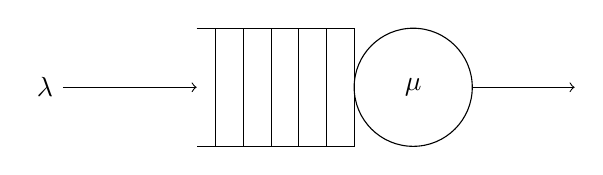
\begin{tikzpicture}
        \draw[->] (-0.7,-0.75) node[left] {\(\lambda\)} -- (1,-0.75);
        \draw (1,0) -- ++(2cm,0) -- ++(0,-1.5cm) -- ++(-2cm,0);
        \foreach \i in {1,...,5}
            \draw (3cm-\i*10pt,0) -- +(0,-1.5cm);
        \draw (3.75, -0.75) circle [radius=0.75cm];
        \node at (3.75, -0.75) {\(\mu\)};
        \draw[->] (4.5, -0.75) -- (5.8, -0.75);
    \end{tikzpicture}

    \vspace{1cm}

    \only<2>{
        \begin{tikzpicture}[-, node distance = 0.7cm]
            \node[state] (zero) {0};
            \node[state, right=of zero] (one) {1};
            \node[state, right=of one] (two) {2};
            \node[state, right=of two] (three) {3};
            \node[state, right=of three, draw=none] (infinity) {\( \dots \)};
            \draw[every loop]
                (zero) edge[bend left] node [above] {\( \lambda \)} (one)
                (one) edge[bend left] node [above] {\( \lambda \)} (two)
                (two) edge[bend left] node [above] {\( \lambda \)} (three)
                (three) edge[bend left] node [above] {\( \lambda \)} (infinity)
                (infinity) edge[bend left] node [below] {\( \mu \)} (three)
                (three) edge[bend left] node [below] {\( \mu \)} (two)
                (two) edge[bend left] node [below] {\( \mu \)} (one)
                (one) edge[bend left] node [below] {\( \mu \)} (zero)
            ;
        \end{tikzpicture}
    }

\end{frame}


\begin{frame}
    \centering
    \frametitle{Queues - M/M/3}
    \begin{tikzpicture}
        \draw[->] (-0.7,-0.75) node[left] {\(\lambda\)} -- (1,-0.75);
        \draw (1,0) -- ++(2cm,0) -- ++(0,-1.5cm) -- ++(-2cm,0);
        \foreach \i in {1,...,5}
            \draw (3cm-\i*10pt,0) -- +(0,-1.5cm);
        \draw (3.75, 0.75) circle [radius=0.75cm];
        \draw (3.75, -0.75) circle [radius=0.75cm];
        \draw (3.75, -2.25) circle [radius=0.75cm];
        \node at (3.75, 0.75) {\(\mu\)};
        \node at (3.75, -0.75) {\(\mu\)};
        \node at (3.75, -2.25) {\(\mu\)};
        \draw[->] (4.5, -0.75) -- (5.8, -0.75);
    \end{tikzpicture}

    \vspace{0.5cm}

    \only<2>{
        \begin{tikzpicture}[-, node distance = 0.7cm]
            \node[state] (zero) {0};
            \node[state, right=of zero] (one) {1};
            \node[state, right=of one] (two) {2};
            \node[state, right=of two] (three) {3};
            \node[state, right=of three, draw=none] (infinity) {\( \dots \)};
            \draw[every loop]
                (zero) edge[bend left] node [above] {\( \lambda \)} (one)
                (one) edge[bend left] node [above] {\( \lambda \)} (two)
                (two) edge[bend left] node [above] {\( \lambda \)} (three)
                (three) edge[bend left] node [above] {\( \lambda \)} (infinity)
                (infinity) edge[bend left] node [below] {\( 3\mu \)} (three)
                (three) edge[bend left] node [below] {\( 3\mu \)} (two)
                (two) edge[bend left] node [below] {\( 2\mu \)} (one)
                (one) edge[bend left] node [below] {\( \mu \)} (zero)
            ;
        \end{tikzpicture}
    }

\end{frame}
